
  
\documentclass[journal,12pt,twocolumn]{IEEEtran}

\usepackage{setspace}
\usepackage{gensymb}
\singlespacing
\usepackage[cmex10]{amsmath}

\usepackage{amsthm}

\usepackage{mathrsfs}
\usepackage{txfonts}
\usepackage{stfloats}
\usepackage{bm}
\usepackage{cite}
\usepackage{cases}
\usepackage{subfig}

\usepackage{longtable}
\usepackage{multirow}

\usepackage{enumitem}
\usepackage{mathtools}
\usepackage{steinmetz}
\usepackage{tikz}
\usepackage{circuitikz}
\usepackage{verbatim}
\usepackage{tfrupee}
\usepackage[breaklinks=true]{hyperref}
\usepackage{graphicx}
\usepackage{tkz-euclide}

\usetikzlibrary{calc,math}
\usepackage{listings}
    \usepackage{color}                                            %%
    \usepackage{array}                                            %%
    \usepackage{longtable}                                        %%
    \usepackage{calc}                                             %%
    \usepackage{multirow}                                         %%
    \usepackage{hhline}                                           %%
    \usepackage{ifthen}                                           %%
    \usepackage{lscape}     
\usepackage{multicol}
\usepackage{chngcntr}

\DeclareMathOperator*{\Res}{Res}
\newtheorem{theorem}{Theorem}[section]
\newtheorem{corollary}{Corollary}[theorem]
\newtheorem{lemma}[theorem]{Lemma}
\newtheorem{definition}{Definition}[section]
\renewcommand\thesection{\arabic{section}}
\renewcommand\thesubsection{\thesection.\arabic{subsection}}
\renewcommand\thesubsubsection{\thesubsection.\arabic{subsubsection}}

\renewcommand\thesectiondis{\arabic{section}}
\renewcommand\thesubsectiondis{\thesectiondis.\arabic{subsection}}
\renewcommand\thesubsubsectiondis{\thesubsectiondis.\arabic{subsubsection}}


\hyphenation{op-tical net-works semi-conduc-tor}
\def\inputGnumericTable{}                                 %%

\lstset{
%language=C,
frame=single, 
breaklines=true,
columns=fullflexible
}
\begin{document}

\newcommand{\BEQA}{\begin{eqnarray}}
\newcommand{\EEQA}{\end{eqnarray}}
\newcommand{\define}{\stackrel{\triangle}{=}}
\bibliographystyle{IEEEtran}
\raggedbottom
\setlength{\parindent}{0pt}
\providecommand{\mbf}{\mathbf}
\providecommand{\pr}[1]{\ensuremath{\Pr\left(#1\right)}}
\providecommand{\qfunc}[1]{\ensuremath{Q\left(#1\right)}}
\providecommand{\sbrak}[1]{\ensuremath{{}\left[#1\right]}}
\providecommand{\lsbrak}[1]{\ensuremath{{}\left[#1\right.}}
\providecommand{\rsbrak}[1]{\ensuremath{{}\left.#1\right]}}
\providecommand{\brak}[1]{\ensuremath{\left(#1\right)}}
\providecommand{\lbrak}[1]{\ensuremath{\left(#1\right.}}
\providecommand{\rbrak}[1]{\ensuremath{\left.#1\right)}}
\providecommand{\cbrak}[1]{\ensuremath{\left\{#1\right\}}}
\providecommand{\lcbrak}[1]{\ensuremath{\left\{#1\right.}}
\providecommand{\rcbrak}[1]{\ensuremath{\left.#1\right\}}}
\theoremstyle{remark}
\newtheorem{rem}{Remark}
\newcommand{\sgn}{\mathop{\mathrm{sgn}}}
\providecommand{\abs}[1]{\vert#1\vert}
\providecommand{\res}[1]{\Res\displaylimits_{#1}} 
\providecommand{\norm}[1]{\lVert#1\rVert}
%\providecommand{\norm}[1]{\lVert#1\rVert}
\providecommand{\mtx}[1]{\mathbf{#1}}
\providecommand{\mean}[1]{E[ #1 ]}
\providecommand{\fourier}{\overset{\mathcal{F}}{ \rightleftharpoons}}
\providecommand{\zee}{\overset{\mathcal{Z}}{ \rightleftharpoons}}
%\providecommand{\hilbert}{\overset{\mathcal{H}}{ \rightleftharpoons}}
\providecommand{\system}{\overset{\mathcal{H}}{ \longleftrightarrow}}
	%\newcommand{\solution}[2]{\textbf{Solution:}{#1}}
\newcommand{\solution}{\noindent \textbf{Solution: }}
\newcommand{\cosec}{\,\text{cosec}\,}
\providecommand{\dec}[2]{\ensuremath{\overset{#1}{\underset{#2}{\gtrless}}}}
\newcommand{\myvec}[1]{\ensuremath{\begin{pmatrix}#1\end{pmatrix}}}
\newcommand{\mydet}[1]{\ensuremath{\begin{vmatrix}#1\end{vmatrix}}}
\numberwithin{equation}{subsection}
\makeatletter
\@addtoreset{figure}{problem}
\makeatother
\let\StandardTheFigure\thefigure
\let\vec\mathbf
\renewcommand{\thefigure}{\theproblem}
\def\putbox#1#2#3{\makebox[0in][l]{\makebox[#1][l]{}\raisebox{\baselineskip}[0in][0in]{\raisebox{#2}[0in][0in]{#3}}}}
     \def\rightbox#1{\makebox[0in][r]{#1}}
     \def\centbox#1{\makebox[0in]{#1}}
     \def\topbox#1{\raisebox{-\baselineskip}[0in][0in]{#1}}
     \def\midbox#1{\raisebox{-0.5\baselineskip}[0in][0in]{#1}}
\vspace{3cm}
\title{QUIZ2}
\author{Adarsh Sai - AI20BTECH11001}
\maketitle
\newpage
\bigskip
\renewcommand{\thefigure}{\theenumi}
\renewcommand{\thetable}{\theenumi}
Download all python codes from 
\begin{lstlisting}
https://github.com/Adarsh541/EE3900/blob/main/quiz2/codes/quiz2.py
\end{lstlisting}

%
Download latex-tikz codes from 
%
\begin{lstlisting}
https://github.com/Adarsh541/EE3900/blob/main/quiz2/quiz2.tex
\end{lstlisting}
\section{Problem(Q3.16(a,b))}
When the input to an LTI system is 
\begin{align}
    x\sbrak{n}=\brak{\frac{1}{3}}^nu\sbrak{n}+\brak{2}^nu\sbrak{-n-1},
\end{align}
the corresponding output is 
\begin{align}
    y\sbrak{n}=s\brak{\frac{1}{3}}^nu\sbrak{n}-5\brak{\frac{2}{3}}^nu\sbrak{n}.
\end{align}
\begin{enumerate}
    \item Find the system function $H\brak{z}$ of the system. Plot the pole(s) and zero(s) of $H\brak{z}$ and indicate the region of convergence.
    \item Find the impulse response $h\sbrak{n}$ of the system.
\end{enumerate}
\section{Solution}
\begin{lemma}\label{l1}
\begin{align}
    a^n u\sbrak{n} &\zee \frac{z}{z-a}, \text{ ROC: }|z|>|a|\\
    -a^n u\sbrak{-n-1} &\zee \frac{z}{z-a}, \text{ ROC: }|z|<|a|\\
    \delta\sbrak{n}&\zee 1, \text{ ROC: }All z
\end{align}
\end{lemma}
\begin{lemma}\label{l2}
\begin{align}
    x\sbrak{n-n_0} \zee z^{-n_0}X\brak{z}
\end{align}
\end{lemma}
\begin{enumerate}
\item Since Z-transform obeys linearity and from Lemma-$\ref{l1}$ 
\begin{align}
    X\brak{z}&=\frac{z}{z-\frac{1}{3}}-\frac{z}{z-2}, \text{ ROC1: } \frac{1}{3}<|z|<2\\
    Y\brak{z}&=5\brak{\frac{z}{z-\frac{1}{3}}-\frac{z}{z-\frac{2}{3}}},\text{ ROC2: } |z|>\frac{2}{3}
\end{align}
\begin{align}
    H\brak{z}&=\frac{Y\brak{z}}{X\brak{z}}\\
    &=\frac{z-2}{z-\frac{2}{3}}\label{eq2}\\
    &=1 - \frac{4}{3}z^{-1}\brak{\frac{z}{z-\frac{2}{3}}}\label{9}
\end{align}
From $\eqref{eq2}$ 
\begin{align}
    Zero &: z=2\\
    Pole &: z=\frac{2}{3}\\
    ROC &: ROC1\cap ROC2\\
    &: \frac{2}{3}<|z|<2
\end{align}
\begin{figure}[!h]
 \centering
 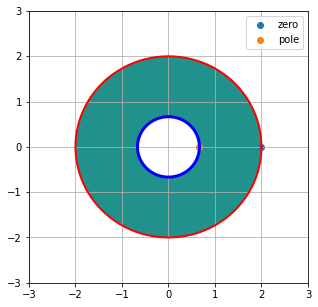
\includegraphics[width=\columnwidth]{quiz2.png}
 \caption{Green region is the ROC.}
\end{figure}
\item From Lemma-$\ref{l1}$, $\ref{l2}$ and $\eqref{9}$ 
\begin{align}
    h\sbrak{n}=\delta\sbrak{n}-\frac{4}{3}\brak{\frac{2}{3}}^{n-1}u\sbrak{n-1}
\end{align}
\end{enumerate}
\end{document}

